\documentclass[msc,lith,english]{liuthesis}

%%%%%%%%%%%%%%%%%%%%%%%%%%%%%%%%%%%%%%%%%%%%%%%%%
% Imports
%%%%%%%%%%%%%%%%%%%%%%%%%%%%%%%%%%%%%%%%%%%%%%%%%
% \usepackage[english]{babel}
\usepackage[utf8]{inputenc}
\usepackage[backend=biber,sorting=none,hyperref]{biblatex}
\usepackage{mathtools}
\usepackage{dsfont}
\usepackage{tikz}
\usetikzlibrary{topaths,calc,tikzmark}
\usepackage{algorithm2e}
\usepackage{pgfgantt}
\usepackage{marginnote}
\usepackage{marvosym}
\usepackage[marginpar]{todo}
\usepackage{pgfgantt}

%%%%%%%%%%%%%%%%%%%%%%%%%%%%%%%%%%%%%%%%%%%%%%%%%
% Settings
%%%%%%%%%%%%%%%%%%%%%%%%%%%%%%%%%%%%%%%%%%%%%%%%%
\department{Institutionen för systemteknik}
\departmentenglish{Department of Electrical Engineering}
\departmentshort{ISY}

\supervisor{Frans Skarman}
\examiner{Oscar Gustavson}
\titleenglish{Wordlength inference and optimization in Spade-lang}
\subtitleenglish{Optimizing your hardware does not have to be hard}
\titleswedish{Ordlängdsinferans i Spade}
\subtitleswedish{Optimering av hårdvara gör det enkelt att vara}
\thesissubject{Datateknik}

\publicationyear{2023}
\currentyearthesisnumber{001}
\dateofpublication{2023-05-20}

\addbibresource{thesis.bib}

\renewcommand{\todomark}{TODO}

\author{Edvard Thörnros}

\begin{document}

%%%%%%%%%%%%%%%%%%%%%%%%%%%%%%%%%%%%%%%%%%%%%%%%%
% Intro
%%%%%%%%%%%%%%%%%%%%%%%%%%%%%%%%%%%%%%%%%%%%%%%%%
\chapter{Introduction}
\label{chaIntro}
\Todo{Is wordlength one word, two or maybe there should be a dash?}
\Todo{I just wrote something, I dislike this}
Computers are a part of our everyday lives and all computers have something that computes, a compute unit. In some cases this is a dedicated CPU but in all cases it can is purpose built hardware. A modern way of building hardware is -- funnily enough -- by writing HDL. If you want to create a special circuit you would not use a general purpose programming language (although subsets of Haskell can compile to hardware \cite{src:ClashExists}), these languages are refered to as Hardware Description Language, or HDL for short. One of these HDL is Spade, a HDL with a focus on usability which borrows much from the modern programming language \cite{src:spadeSomething} \cite{src:spadeAnHDL}. By writing high level code when describing hardware, we also open the door for optimizations and help from the compiler. This is the topic of this master thesis, a specific kind of optimization and user-help that can make Spade faster and safer.

This thesis focus on a specific kind of optimization, wordlength inference. Using a novel approach of combining wordlength inference with type inference. Wordlength is the number of bits to allocate to a value and when creating hardware you often have to specify this yourself. Getting this wordlength right everywhere can be tedious and time consuming. A small error in the wordlength might cause faults in the program and a too large wordlength wastes resources. %% \cite{src:BugsWithWordLength}. %% Some sources would be lovely here
Since the compiler has access to all the source code for the hardware, the compiler should be able to check the wordlengths everywhere and potentially optimize the wordlength where bits go unused. Putting these optimizations in the compiler allows code to be more general and easier to reuse, a common good practice in the software industry today. 

\section{Motivation}
Creating more powerful tools allows us to do more powerful things with them. In the case of software this effect is even larger, anyone with a laptop and a dream can develop programs for anyone to use. One of these fundamental tools is the compiler and programming languages -- no one in their right mind would use FORTRAN today when they have alternatives like Go, Rust or Python. Bringing this mindset to the hardware world could increase the productivity, usability and accessibility to custom circuits and accelerators. HDLs have the huge potential of improving all computation speeds in the world. It's questionably if this thesis alone will take us as far as to revolutionize the hardware industry, but it's certainly a step in the right direction for energy-efficient and faster computations.

\section{Research questions}
\begin{enumerate}
  \item How can interval arithmetic and affine arithmetic be used to implement wordlength inference?
  \item How does wordlength inference and optimization affect the number of LUTs, DPS-blocks and memories for a circuit?
  \item Can wordlength inference be used to create more reusable code?
\end{enumerate}

\section{Aim}
This thesis will implement wordlength inference in the Spade compiler using a combination of interval arithmetic and affine arithmetic. The implementation should then be evaluated using a synthesis tool and compared to other Spade-programs without these optimizations.

\section{Delimitations}
The sample size of the programs is quite limited, there is no attempt made to generalize the findings to all hardware. This thesis is limited to Spade and FPGAs and will not consider optimizations on other kinds of hardware. Other more sophisticated error-estimation like ME-gPC will not be studied.

%%%%%%%%%%%%%%%%%%%%%%%%%%%%%%%%%%%%%%%%%%%%%%%%%
% Background
%%%%%%%%%%%%%%%%%%%%%%%%%%%%%%%%%%%%%%%%%%%%%%%%%
\chapter{Background}
\label{chaBackground}
A sufficient basis to understand this work is presented in this chapter.

% Programming languages in general is considered one of the more mature topics in computer science. There are many, many books and papers written on compilers. Some programmers even consider compilers to be black boxes which they must obey, frightened of the complexities and details of the black magic working inside. This background aims to unbox these beasts called compilers and shed some light on them. Explaining all the details of a compiler and the typechecker is out of scope for this background.
% 
% Wordlengths, HDLs and also get a section describing how they fit into this work.


\section{Introduction to Compiler Structure}
What constitutes a compiler is not always obvious. A compiler, in the most banal sense, takes an input program and outputs an output program. Some want the output to be ``simpler`` than the input, passing in a high level program in C and outputting executable X86 machine code where X86 is considered a ``simpler`` than C. The input to the compiler is often text, and we will assume this for the rest of this short introduction to compilers.

Each compiler is unique, but they often have a shared structure. The first step is often to do lexical analysis (also called lexing) in a lexer or tokenizer. Here characters are abstracted away, and the compiler has done the first processing of the text. When lexing you often decide what piece of text is an integer-constant, a keyword, a string, etc. After the lexing the tokens are used to perform semantic analysis -- parsing. During parsing the compiler understands structures in the program such as what is part of each function or correctly parsing the order of operations for mathematical expressions. The parsing usually produces an abstract syntax tree. Though some compilers interweave these steps, they are usually there in spirit.

The Spade compiler has both a lexer step and a parser step which are located in different modules.

The compilers work is not done yet. After all the syntactical analysis the semantic analysis can be started, semantic analysis is sometimes referred to as the ``inner layers of the compiler``. Here we resolve identifiers, run type-checking and other static program analysis or do optimizations like moving around constants to avoid needless copies. The wordlength inference and optimizations will be an inner layer, the relevant details will be discussed in the Section \ref{sec:TypeChecking}. 

After the compiler has finished optimizing, the output is generated and potentially lowered (made less complex) in multiple stages, often by translating to a simpler internal representation which in the end makes generating the final output of the compiler easier.

One ``layer`` is often called a ``pass``. Spade is not a multi-pass compiler and perform these steps sequentially -- not interleaved.
\cite{src:DragonBook}\cite{src:CraftingInterp}\cite{src:KKLectures}

\begin{figure}
\begin{center}
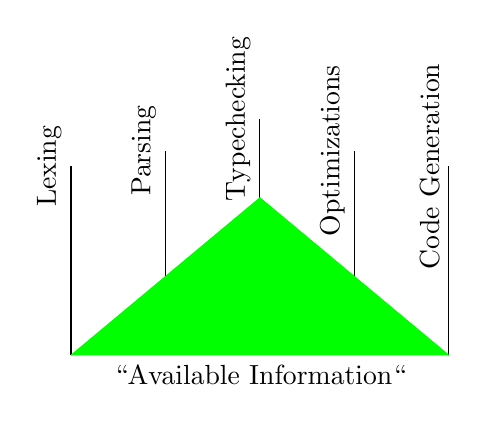
\begin{tikzpicture}[xscale=3, yscale=2]
% vertical lines
\draw (0,0) -- (0,1.2) node[above, rotate=90] {Lexing};
\draw (0.4,0) -- (0.4,1.3) node[above, rotate=90] {Parsing};
\draw (0.8,0) -- (0.8,1.5) node[above, rotate=90] {Typechecking};
\draw (1.2,0) -- (1.2,1.3) node[above, rotate=90] {Optimizations};
\draw (1.6,0) -- (1.6,1.2) node[above, rotate=90] {Code Generation};
% horizontal line
\filldraw[color=green, fill=green] (0,0) -- (0.8,1.0) -- (1.6,0);
\draw (0.8,0.0) node[below] {``Available Information``};
\end{tikzpicture}
  \caption{A visualization of the rough measurement of information present in each step of the compilation process. Typechecking having the most information and lexing and code generation having the least amount of information.}
  \label{fig:InformationCompilation}
\end{center}
\end{figure}

Compilers have to construct a lot of complex information about the program. A visual that I find helpful when reasoning about compilers is an imagined graph of ``available information``. Figure \ref{fig:InformationCompilation} tries to communicate the amount of information created in each step of compilation. The most important part being that we know a lot about the program in the type checking phase.

\section{Type Checking} % Maybe `inner layers`?
\label{sec:TypeChecking}
Type checking is a way of making sure the program is internally consistent, there are no contradictions inside to program to the program itself. Type checking can be done in different ways with different pros, cons or preferences \cite{src:TypeCheckersBook}. The typechecker in Spade can infer types and deduce things about the program, like ``the first argument is a 3-bit integer value, but you gave a record`` \cite{src:spadeAnHDL}. Typechecking has shown to reduce some kinds of programming errors and can in some cases even suggest what functions to use.

The typechecker in Spade is a one directional Damas–Hindley–Milner typechecker. This means it stops on the first error and can deduce types to their most general form. So if asked to typecheck the identity function (a function that takes one value and returns the value as is, the function does nothing) the typechecker would be able to deduce that the argument could have any type, but that the type is the same as the return value, without any help from the programmer except the body of the function. \cite{src:DamasHindleyMilner}


\section{Interval Arithmetic and Affine Arithmetic}
\label{sec:IAandAA}

There is an excellent explanation of both Interval- and Affine Arithmetic by \citeauthor{src:affAri} -- the following section is a short version to cover the absolute basics of the material.

Affine arithmetic and interval arithmetic and two common ways to estimate. They can be applied to estimating the number of piano tuners in Chicago \cite{src:pianoTuners} or the cosine of an angle. They also have a place in static analysis of programs, which is the focuses of this thesis. This section describes what these concepts are, references literature if you want to read more and shows their roll in static analysis of programs. These methods are often referred to as over-estimation.

Though affine arithmetic is more sophisticated it does not always produce better results, interval arithmetic can for some computations produce tighter bounds. There are other methods that are considered more sophisticated like ME-gPC, but the extra complexity can be added later if it is found to be needed.

\subsection{Interval Arithmetic}
Interval arithmetic operates on intervals, as the name implies. A value -- or in the context of a program, a variable -- has a smallest and largest value it can assume. Consider \verb`x = random\_real()`, where \verb`random_real` generates a random value in the range $[0, 1]$. We can express this in interval arithmetic as $\bar{x} = [0, 1]$, intervals will be denoted with a bar on top to separate them from the variables. Note especially that the true value of $x$ lies in the interval $\bar{x}$. In this example we know $0 \leq x \leq 1$, also written as $x \in [0, 1]$. These intervals can be added, negated, and so on, to give you an estimate of an arbitrary expression.

For a more throughout guide I recommend (INSERT SOURCE HERE)[self-validated-numerical-methods-and-applications], this section will cover the basics that are needed to understand the concept and understand this thesis. A full description of the field is out of scope.

\subsubsection{Interval Arithmetic Special values}
When doing static program analysis, some extra values are often defined. For example, it's okay to have an interval where one value is infinite. This interval is perfectly valid $[5, \infty]$.

The empty interval is also defined, $[]$. This interval usually denotes expressions or code that cannot be reached or evaluated. It might seem useless at a glance, but is required to do more sophisticated static analysis.
\Todo{IA, I have shorter definitions written in ``affine-and-interval-arithmatic.md``, but I think I'll just refer to the original sources since it's not really relevant except for the implementation, unless I get a specific result due to one of them.}

\subsubsection{Interval Arithmetic: An example and Limitations}
I find that one of the best ways to understand these things is with an example.
We will be using the expression $2x + z - z$ as an example where $x = [0, 1], z = [1, 3]$.

\Todo{Make this clearer, I feel the understanding is lacking}
\begin{verbatim}
2 * [0, 1] + [1, 3] - [1, 3]
// Scaling rule and subtraction is negated addition 
[2 * 0, 2 * 1] + [1, 3] + (-1 * [1, 3])
// Calculate
[0, 2] + [1, 3] + [-3, -1]
// Sum it upp
[-2, 4]
\end{verbatim}

This gives us the conclusion that this expression will lie in the range $[-2, 4]$ for the given values of $x$ and $z$. This is true, but the estimate is larger than it necessarily needs to be. An observant reader would notice that subtracting the value $z$ from itself should result in $0$, which is a perfectly valid point. This is a limitation of the interval arithmetic. Interval arithmetic doesn't reason about the expressions that came before it and how they combine, and this limitation would exist if used to do static analysis of programs. But this limitation leads us to affine arithmetic, which lets us reason more about the expressions we evaluate.


\subsection{Affine Arithmetic}
Affine arithmetic (AA) works similarly to interval arithmetic (IA), but has a memory of where values come from and can reason about their combinations at a higher level. That said, AA does not produce strictly better results than IA in all circumstances and a combination is currently thought to be the current state of the art. 

\subsubsection{How Affine Arithmetic works}
In affine arithmetic there's a concept of noise symbols ($e_i$ where $i$ is a natural number) and the numbers half width ($x_i$ where $i$ is a natural number). A linear combination of these noise symbols is a reasonable way to represent a "number" when reasoning about affine arithmetic, $\hat{x} = x_0 + x_1e_1 + x_2e_2 + \dots$. These terms can them be combined using similar rules to interval arithmetic.

Notice how the first term lacks a noise symbol, this expresses where the center of the uncertainty is. The different noise variables serve as the memory of this expression, consider subtracting $\hat{x} - \hat{x}$ with itself we get the expected result of 0 from that.

\subsection{Error Explosion for Affine- and Interval Arithmetic }

% Both AA and IA accumulate error in order to overestimate. If this error gets too large, the estimations become so vague the estimation is useless. The more operations that are being estimated the larger this error gets. Luckily this doesn't affect the correctness only the error of the answer but if the error is too large the estimation becomes useless.

\cite{src:affAri}

\Todo{Modified Affine Arithmetic?}
\Todo{A nice image here would help understanding}

\section{Wordlength inference}
\Todo{Explain what it is and why it exists}


\section{Spade}
\Todo{Explain what it is and why it exists, also shove some syntax}

\section{FPGA}
\Todo{Explain what an FPGA is and what makes it different from micro controllers}

%%%%%%%%%%%%%%%%%%%%%%%%%%%%%%%%%%%%%%%%%%%%%%%%%
% Related Work
%%%%%%%%%%%%%%%%%%%%%%%%%%%%%%%%%%%%%%%%%%%%%%%%%

\chapter{Related Work}
\Todo{Needs a lot more content here, and it's a very well studied subject}

\section{Minimization of Fractional Wordlength on Fixed-Point Conversion for High-Level Synthesis}
Minimization of Fractional Wordlength on Fixed-Point Conversion for High-Level Synthesis suggests a method for using as few bits in the fractional part of values as possible. Their approach resulted in decent optimizations and was much faster than doing the optimization by hand. The sample size of the programs is quite small and didn't always show as promising results.

\cite{src:MinOfFrac}

\section{High-level synthesis and arithmetic optimizations}
The thesis ``High-level synthesis and arithmetic optimizations`` is an attempt to merge the fields of arithmetic with and HDL-compilers. Several approaches are evaluated that affect correctness, throughput and latency. It describes fixed-point and floating point arithmetic, FPGA hardware and FPGA optimizations in a very clear way.

Problems with the IEEE floating point numbers are mentioned, for one how the implicit rounding causes addition to be non-associative, and how C/C++ compilers used for HDL use CPU optimizations which aren't always suitable for FPGA.

\citeauthor{src:HLSandOpt} is an alternative approach to Spade when it comes to generating hardware and it tries to generate better FPGA hardware by modifying a compilation layer for the current compilers. But C/C++ has a fundamental problem when being mapped to hardware, the languages were built for single-threaded sequential computations where FPGAs prefer to do computations in parallel.

\cite{src:HLSandOpt}

% # Planned literature supporting the thesis
% - Books and papers on IA and AA
%   - Self-Validated Numerical Methods and Applications
% - Static analysis books and literature, potentially digging into bounded model checking (BMC) and the likes
%   - Calculus of Computation, maybe more literature here
% - The course on program analysis available on LiU 
%   - TDDE34 and the presentations there
% - Previouse literature on Spade
%   - Spade: An HDL Inspired by Modern Software Languages and co
% - Books and papers on typecheckers and compilers books and literature
%   - Some papers on Henk are interesting
%   - Complete and Easy Bidirectional Typechecking for Higher-Rank Polymorphism
%   - Types and Programming Languages by Ben Pierce
% - There's a lot of FPGA literature on FPGA optimizaton, here are a few I've seen 
%    - Constantinides, George A.
%      Word-length Optimization for Differentiable Nonlinear Systems
%    - N. Doi and T. Horiyama and M. Nakanishi and S. Kimura
%      Minimization of fractional wordlength on fixed-point conversion for high-level synthesis
%    - I have like 10 more of these...


%%%%%%%%%%%%%%%%%%%%%%%%%%%%%%%%%%%%%%%%%%%%%%%%%
% Project Plan
%%%%%%%%%%%%%%%%%%%%%%%%%%%%%%%%%%%%%%%%%%%%%%%%%
\chapter{Project Plan}
A brief outline of the project and what I'm to do is described.

\section{Method idea}
The method sketch looks like this:
\begin{enumerate}
  \item Implement wordlength deduction in Spade
  \item Implement wordlength minimization in Spade
  \item Make the wordlength deduction toggleable
  \item Find ~8 programs that represent a vide usage of Spade features
  \item Simulate the programs and make sure they behave identically
  \item Run a synthesis tool on the 8 programs with and without the wordlength deduction in a synthesis-tool. Note down the LUT usage, the expected power draw. The data gathered is the control data.
  \item Compare the results.
  \item Profit.
\end{enumerate}

\section{Expected Results}
I expect to find places where the wordlength could be deduced and optimized. I expect no effect on correctness. In simple applications the inference should result in better wordlengths and decreased resource usage. The greatest gain I expect is in the code re-usability.

\newpage
\section{GANTT-chart}

\begin{center}
\begin{figure}[htp]
\begin{ganttchart}[
    vgrid,
    bar left shift=0.15,
    bar right shift=-0.15,
    bar/.append style={rounded corners=3pt},
    bar inline label node/.style={%
      anchor=south, font=\ganttvalueof{bar label font}%
    },%
    inline,
    milestone inline label node/.style={%
      anchor=north, font=\ganttvalueof{milestone label font}%
    },%
    expand chart=\textwidth
]{1}{20}
\gantttitle{Project Plan}{20} \\
\gantttitlelist{1,...,20}{1} \\

\ganttbar{Scope project}{1}{3} \\
\ganttmilestone{The plan for the thesis}{3} \\

\ganttgroup{Implementation}{4}{13} \\
\ganttbar{Plan implementation}{4}{4}
\ganttbar{Write code}{5}{11}
\ganttbar{Evaluation}{12}{13}

\ganttmilestone{Version of WL-inference that can be demoed}{8} \\
\ganttmilestone{Preliminary results}{11} \\

\\
\ganttgroup{Thesis}{1}{19} \\
\ganttbar{Background}{1}{10}
\ganttmilestone{Find opponent}{16} \\

\ganttmilestone{1st hand in}{17}
\ganttbar{Related works}{4}{10} \\
\ganttbar{Method}{3}{5}

\ganttbar{Results}{11}{13}
\ganttbar{Conclusion}{15}{16} \\

\ganttbar{Discussion}{14}{15}
  \ganttbar{Polish report}{17}{17} \\
\ganttbar{Presentation}{18}{20} \\

\ganttmilestone[milestone inline label node/.style={anchor=north east}]{Hold presentation and final hand in}{20} \\

\ganttgroup{Research}{1}{8} \\
\ganttbar{Read papers}{1}{8} \\

% \ganttlink{elem11}{elem12}
% \ganttlink{elem11}{elem4}
% \ganttlink{elem5}{elem12}
% \ganttlink{elem10}{elem12}
% \ganttlink{elem9}{elem12}
% \ganttlink{elem22}{elem9}
% \ganttlink{elem22}{elem10}
% \ganttlink{elem7}{elem8}
% \ganttlink{elem6}{elem7}
% \ganttlink{elem8}{elem9}
% \ganttlink{elem9}{elem10}
\end{ganttchart}
  \caption{The project plan for the thesis project.}
  \label{figGanttChart}
\end{figure}
\end{center}

\subsection{Scope project}
Understand what the project is and what the goal (and ant-goals) of the project are. What kind of implementation is needed? Are there simpler ways of reaching the same goal? These kinds of questions are answered and result in the thesis plan.

\subsection{Implementation}
The project will contain implementation. During the implementation section, program code is changed to make the changes needed to the codebase.

\subsection{Plan implementation}
Here we decide how to implement what needs to be implemented. This will result in some kind of specification or more detailed plan that can be used as a jumping off point.

\subsection{Write code}
Here code is written to add the needed features to the compiler.

\subsection{Evaluation}
Here we look for problems with the implementation and run evaluations on the compiler to measure the difference in resource usage. 

\subsection{Thesis}
This section is all about the written thesis which is produced for this project.

\subsection{Background}
The background is written here.

\subsection{Related works}
Related works section is written here.

\subsection{Method}
The method is written and planned here.

\subsection{Result}
The result is written here.

\subsection{Conclusion}
The conclusion is written here

\subsection{Discussion}
The conclusion is written here

\subsection{Polish report}
The report is cleaned up and read through -- clearing up what needs to be clearing up.

\subsection{Presentation}
The presentation is worked on in this section.

\subsection{Research}
This section is for understanding the field and researching

\subsection{Read papers}
Papers in the field are read to understand the field more deeply and figure out how and what needs to be done.

\section{Resources}
I need access to FPGA simulation and synthesis software.

\section{Risks}

\newcommand{\riskHeader}[2]{(\textbf{likelihood:} #1, \textbf{severity:} #2)}
\begin{enumerate}
  \item \riskHeader{medium}{medium} A compiler is a complex piece of software, I might miss something important when integrating my changes and this might cause the implementation to take extra time. I can mitigate this by adding extra slack time in the plan for development.

  \item \riskHeader{low}{high} There are limitations to Damas–Hindley–Milner typesystems and things that cannot be done with them. Maybe wordlength induction interacts poorly with the typechecker and bug or other incorrect behavior might sneak in.

  \item \riskHeader{medium}{low} Software might be hard to gauge the progress of if you don't understand all the details involved. I might have trouble communicating my progress or where I am in the development cycle. I can mitigate this by doing small commits and bundles of work that can be integrated early to show some kind of progress.

  \item \riskHeader{medium}{high} I might work less than I plan each week due to other things in my life, unfortunately I can't plan around then only for them. This is extra prevalent since I feel like I've already done half a thesis. This will most likely drain my motivation and might result in me not finishing the thesis and getting my degree. Only mitigation I know of is to have fun, but this problem cannot be avoided or solved.

\end{enumerate}

\printbibliography

\todos

\end{document}
